% $Header: /cvsroot/latex-beamer/latex-beamer/solutions/generic-talks/generic-ornate-15min-45min.en.tex,v 1.5 2007/01/28 20:48:23 tantau Exp $

\documentclass{beamer}

% This file is a solution template for:

% - Giving a talk on some subject.
% - The talk is between 15min and 45min long.
% - Style is ornate.



% Copyright 2004 by Till Tantau <tantau@users.sourceforge.net>.
%
% In principle, this file can be redistributed and/or modified under
% the terms of the GNU Public License, version 2.
%
% However, this file is supposed to be a template to be modified
% for your own needs. For this reason, if you use this file as a
% template and not specifically distribute it as part of a another
% package/program, I grant the extra permission to freely copy and
% modify this file as you see fit and even to delete this copyright
% notice. 

\mode<handout>{
  \usepackage{pgfpages}
  \pgfpagesuselayout{4 on 1}[a4paper,border shrink=5mm]
}
\mode<presentation>{	
  \usetheme{Warsaw}
  \setbeamertemplate{caption}[numbered]
}
\usepackage{url}
\usepackage[english]{babel}
% or whatever
\usepackage{fancybox}
\usepackage[latin1]{inputenc}
% or whatever

\usepackage{times}
\usepackage[T1]{fontenc}
% Or whatever. Note that the encoding and the font should match. If T1
% does not look nice, try deleting the line with the fontenc.


\title % (optional, use only with long paper titles)
{Soft Errors}

\subtitle
{A curse from the heavens} % (optional)

\author % (optional, use only with lots of authors)
{Smruti R. Sarangi}
% - Use the \inst{?} command only if the authors have different
%   affiliation.

\institute[Universities of Somewhere and Elsewhere] % (optional, but mostly needed)
{
  Department of Computer Science\\
  Indian Institute of Technology \\
  New Delhi, India 
}
% - Use the \inst command only if there are several affiliations.
% - Keep it simple, no one is interested in your street address.
\date{}
\subject{Lectures}
% This is only inserted into the PDF information catalog. Can be left
% out. 

\renewcommand{\raggedright}{\leftskip=0pt \rightskip=0pt plus 0cm} 

% If you have a file called "university-logo-filename.xxx", where xxx
% is a graphic format that can be processed by latex or pdflatex,
% resp., then you can add a logo as follows:

% \pgfdeclareimage[height=0.5cm]{university-logo}{university-logo-filename}
% \logo{\pgfuseimage{university-logo}}



% Delete this, if you do not want the table of contents to pop up at
% the beginning of each subsection:
\AtBeginSubsection[]
{
  \begin{frame}<beamer>{Outline}
    \tableofcontents[currentsection,currentsubsection]
  \end{frame}
}


% If you wish to uncover everything in a step-wise fashion, uncomment
% the following command: 

%\beamerdefaultoverlayspecification{<+->}


\begin{document}

\begin{frame}
  \titlepage
\end{frame}

% This is the main Outline Section
\begin{frame}{Outline}
  \tableofcontents
  % You might wish to add the option [pausesections]
\end{frame}

\section{Introduction}

\begin{frame}{Curse from the Heavens}
 \begin{figure}[h]
  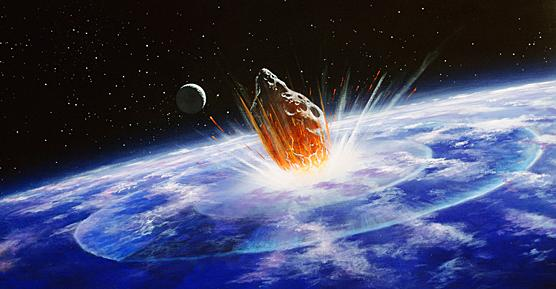
\includegraphics[width=4in]{meteorite}
 \end{figure}

\end{frame}

\begin{frame}[shrink=25]{Soft Error}
\begin{figure}[h]
 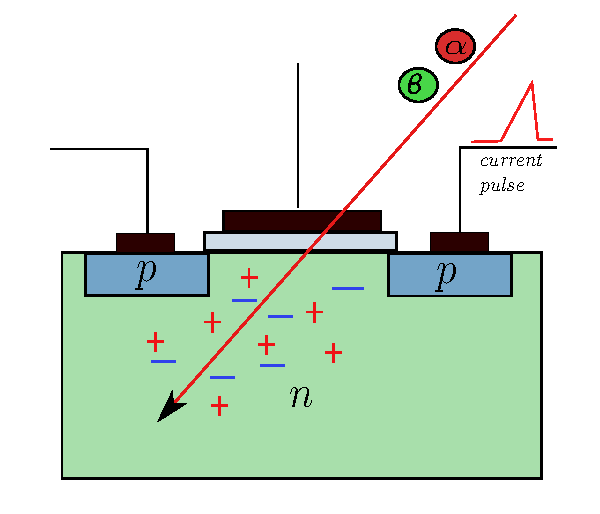
\includegraphics[width=2.5in]{seu}
  \caption{\footnotesize Current pulse after a particle strike}
\end{figure}
	
\begin{definition}{Soft Error:}
  A {\color{red} soft error} is any measurable or observable change in state or performance of a microelectronic 
    device, component, subsystem, or system (digital or analog) resulting from 
    a single energetic particle strike. The particle includes but is not limited to alpha particles,
    neutrons, and cosmic rays.
\end{definition}

\end{frame}

\begin{frame}[shrink=10]{History of Research in Particle Strikes}
 \begin{itemize}
  \item People recorded failures in above ground nuclear sites from 1954 to 1957. (Wallmark and Marcus, 1962)
  \item They started becoming important in space missions in the seventies.
  \item The first example of soft errors in circuits was observed in DRAMs. This was observed for the first time
	at sea level.
  \item In the early 80s most of the soft errors used to happen because of traces of radioactive elements like uranium and thorium
        in the packaging materials.
  \item Soft Errors gradually started affecting static RAMs. The failure rate is between 100 to 1000 FITs. 
  \item By 2012, soft errors will begin affecting logic circuits. (adders, multipliers, and other complex units).
 \end{itemize}
\end{frame}

\begin{frame}{Types of Soft Errors}
  \begin{itemize}
   \item Intrinsic
      \begin{itemize}
	\item Power supply noise, cross coupling noise.
	\item Temperature variations.
      \end{itemize}
    \item Extrinsic
      \begin{itemize}
	\item Cosmic rays.
	\item alpha particles, neutrons, neutrinos, gluons
      \end{itemize}
  \end{itemize}

\end{frame}

\section{Mechanism}
\begin{frame}[shrink=5]{Radiation Mechanisms in Semiconductors}
 \begin{itemize}
  \item {\color{blue} Alpha Particles:} In the 70s the were emitted by traces of uranium and thorium impurities in packaging materials. Gold used in the pins 
and lead based isotopes in solder bumps are mainly responsible for alpha particle emissions today. Their energy is between 4-9 MeV. 
  \item {\color{blue} Neutrons: } These are produced by cosmic interactions in far away galaxies. They are able to penetrate the earth's atmosphere and ionize
  the silicon substrate. Their energy is about 1 MeV. 
  \item {\color{blue} Secondary radiation:} Alpha particles and lithium nuclei are produced by the interaction of neutrons with the unstable isotope of boron, 
$B^{10}$, in boron doped silicon. Their
energy is approximately 1 MeV. They were the major source of soft errors in 25 and 18 $\mu$ technologies. However, $B^{10}$
is nowadays filtered out in the fabrication process.
 \end{itemize}
\end{frame}

\begin{frame} {Dynamics of a Strike}
 \begin{itemize}
  \item In CMOS circuits the transistors in an ``off'' state are the most sensitive to particle strikes.
    \item Sensitive areas.
      \begin{itemize}
	\item Channel region of the nmos transistor.
	\item Drain region of the pmos transistor.
      \end{itemize}

  \item The particles typically have an LET greater 20 MeV -- $cm^2$/mg. 
 \end{itemize}
\begin{definition} {Linear Energy Transfer (LET)}
 It is the amount of energy that a particle dissipates per unit distance. It is typically divided by the 
density of the target material.
\end{definition}
\end{frame}

\begin{frame}{What Happens on a Strike}
\begin{itemize}
  \item The particle displaces electrons and holes, thus ionizing a part of the silicon substrate.
\pause
  \item The displaced electrons and holes begin to recombine. This creates a current pulse.
\pause
  \item The current pulse propagates to other parts of the circuit. When the displaced charge, {\color{blue}{$Q_{coll}$}} , is more than {\color{blue}{$Q_{crit}$}}, the pulse
      is large enough to create a change in state.
\pause
  \item $Q_{coll}$ is a function of the ionizing particle's energy, trajectory, point of impact, and the local electric field. 
\pause
  \item The current transient lasts for around 200 picoseconds. (NOTE: A clock cycle is 500 ps on a 2 GHz processor). Most of the impact 
	is within 2-3 microns of the impact site.
\end{itemize}
\end{frame}

\begin{frame}{Shape of the Pulse}
\begin{itemize}
 \item The current pulse typically has a sharp rise, and a very gradual fall.
\end{itemize}

\begin{equation*}
 I(t) = \frac {Q_{coll}}{\tau_\alpha - \tau_\beta} \left ( e^{-\frac{t}{\tau_\alpha}} - e^{-\frac{t}{\tau_\beta}} \right )
\end{equation*}

\begin{itemize}
 \item $\tau_\alpha$ is the collection time constant, which is process dependent.
  \item $\tau_\beta$ is the ion-track establishment time constant. This is independent of technology. 
   \item Typical values : $\tau_\alpha$ = 164 ps, $\tau_\beta$ = 50 ps
  \item The displaced charge is about 0.65 pC. 
\end{itemize}

\end{frame}

\begin{frame}[shrink=10]{Shape of the Pulse-II}
 \begin{figure}[h]
  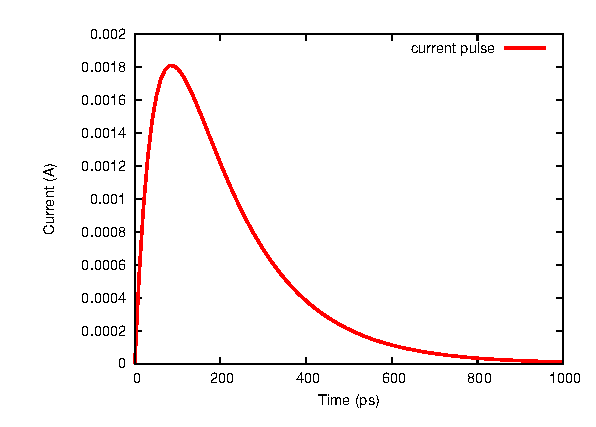
\includegraphics[width=3in]{pulse}
  \caption{\footnotesize A typical current pulse}
 \end{figure}
\begin{itemize}
 \item Any kind of heavy tailed distribution can be used to model it.
    \begin{itemize}
      \item Pareto, Log-Normal, Weibull, Double Exponential, Levy
    \end{itemize}
\end{itemize}
\end{frame}

\begin{frame}[shrink=5]{Hazucha-Svensson Model}
\begin{itemize}
 \item Let us define the term {\em SER} as the number of times a current pulse capable of flipping a bit is generated per second.
  \item The Hazucha-Svensson model defines the SER to be 
    \begin{equation*}
      SER = F * CS
    \end{equation*}
    \begin{itemize}
      \item $F$ is the neutron flux. The number of neutrons hitting an unit area per second.
      \item $CS$ : Critical Section. This is the area that is susceptible to particle strikes. 
    \end{itemize}
  \item The critical section, $CS$, is proportional to the drain area and is an inverse exponential function of $Q_{crit}$
      \begin{equation*}
	CS \propto A * e^{-\frac{Q_{crit}}{Q_S}}
      \end{equation*}
\end{itemize}
\end{frame}

\begin{frame}{Hazucha-Svensson Model II}
 \begin{itemize}
  \item $Q_S$ is the called the {\em collection slope}
  \item It depends on the supply voltage and the doping profile.
 \end{itemize}

The Hazucha-Svensson model proposes a one parameter model for the shape of the pulse.
\begin{equation*}
 I(t) = \frac{2}{T \sqrt{\pi}} \sqrt{\frac{t}{T}} e^{-\frac{t}{T}}
\end{equation*}

\begin{itemize}
 \item $T$ is called the effective parameter. 
\end{itemize}

\end{frame}

\section{Prevention and Recovery}
\begin{frame} {General Approaches}
 \begin{itemize}
  \item Device Level Solutions
  \item Circuit Level Solutions
  \item Architecture Level Solutions
 \end{itemize}

\end{frame}

\subsection{Device Level Solutions}
\begin{frame}{Purification of the Silicon}
  \begin{itemize}
   \item Use low alpha packaging materials.
      \begin{itemize}
	\item Uranium and Thorium impurities are reduced to less than 100 parts per trillion.
	 \item Purify the gold connectors. Use low alpha based lead isotopes for the soldering.
      \end{itemize}
\pause
    \item Reduced the incidence of $B^{10}$.
      \begin{itemize}
	\item Check all dopants for the unstable isotope.
	\item Replace Boron Phosphate Silicate Glass (use as an insulator between metal layers) with other insulators.
      \end{itemize}

  \end{itemize}

\end{frame}

\begin{frame}{Use Radiation Hardened Processes}
\begin{itemize}
 \item There are two broad approaches to solving this problem: Reduce $Q_{coll}$ or increase $Q_{crit}$.
 \item Reduce $Q_{coll}$
    \begin{itemize}
	\item Use a triple well process
	\item Silicon on insulator process
    \end{itemize}
  \item Increase $Q_{crit}$
    \begin{itemize}
	\item Increase the supply voltage of the transistor
	\item Increase the size of the transistor
    \end{itemize}
  
\end{itemize}
\end{frame}

\begin{frame}[shrink=10] {Triple Well Process}
\begin{center}
 \begin{figure}[h]
  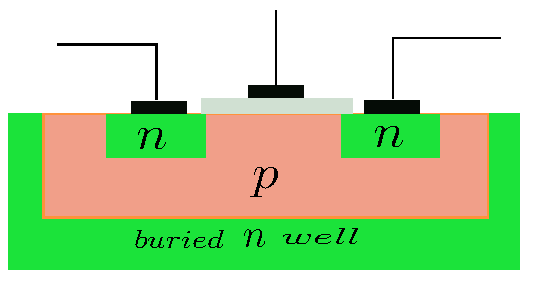
\includegraphics[width=3in]{triple_well}
  \caption{\footnotesize Triple-well process for a NMOS transistor}
 \end{figure}
\end{center}
\begin{itemize}
 \item An extra n-layer is added to isolate the substrate from electrical interference.
  \item It is also very effective in reducing the displaced charge.
\end{itemize}

\end{frame}

\begin{frame}[shrink=10]{ Do you know the name of this stone?}

\begin{center}
 \begin{figure}[h]
  
\includegraphics[width=2in]{sapphire}
 \end{figure}
\end{center}
\pause
\centering{
\alert{Sapphire} }

\end{frame}

\begin{frame}[shrink=10]{Silicon on Insulator(SOI)}
 \begin{center}
 \begin{figure}[h]
  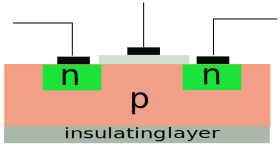
\includegraphics[width=2in]{soi}
  \caption{\footnotesize SOI based NMOS transistor}
 \end{figure}
\end{center}
\begin{itemize}
 \item The insulator is sapphire if we desire a radiation hardened process.
  \item The insulator shields the substrate from an external influence. 
  \item It also decreases its net volume, thus decreasing $Q_{coll}$ in the process.
\end{itemize}
\end{frame}

\begin{frame}[shrink=5]{All about $Q_{crit}$}
 \begin{itemize}
  \item $Q_{crit}$ primarily depends on four factors
      \begin{itemize}	
	\item Transistor size
	\item Supply voltage
	\item Output capacitance
	\item Doping Density
      \end{itemize}
 \end{itemize}
\begin{itemize}
 \item $Q_{crit}$ decreases almost linearly with an increasing $W/L$ ratio. 
  \item $Q_{crit}$ decrease very sharply with an increase in supply voltage. 
\end{itemize}
\end{frame}

\subsection{Circuit Level Techniques}

\begin{frame} {Logical Masking}
\begin{figure}[h]
 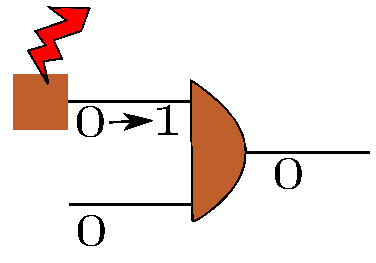
\includegraphics[width=3in]{logical_masking}
\end{figure}
\end{frame}

\begin{frame}[shrink=3]{Electrical Masking}
 \begin{figure}[h]
  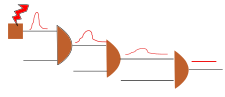
\includegraphics[width=2.5in]{electrical_masking}
  \caption{\footnotesize Electrical masking : Pulse attenuation}
 \end{figure}


\begin{itemize}
 \item A pulse gets severely attenuated as it passes through multiple gates.
 \item It gradually loses all of its energy. 
\end{itemize}
\end{frame}

\begin{frame}{Timing Window Masking}
 \begin{center}
  \begin{figure}[h]
    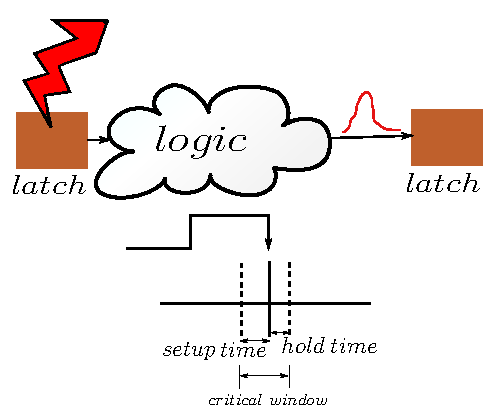
\includegraphics[width=3in]{timing_window_masking}
  \end{figure}
 \end{center}
\end{frame}

\begin{frame}{Finding Sensitive Latches and Gates}
 \begin{itemize}
  \item Find the set of latches that are on sensitive paths. A ``sensitive path'' is a path of logic gates
that can propagate a soft error with high probability.
    \begin{itemize}
      \item Increase the size of the transistors of the latch.
      \item Increase the output capacitance of the latch.
    \end{itemize}
\pause
  \item Find the set of logic gates that are on sensitive paths. 
    \begin{itemize}
      \item Increase the chances of electrical masking by increasing the size of the transistors in the gate.
      \item Or, connect those to a higher supply voltage line.
    \end{itemize}

 \end{itemize}

\end{frame}

\subsection{Architecture Level Techniques}

\begin{frame}{ECC and Redundancy}
 \begin{itemize}
  \item ECC : Error Correction Code
    \begin{itemize}
    \item We typically have a SECDED code (single error correction, double error detection)
    \item Almost all the memory elements are protected
      \begin{itemize}
	\item {\color{blue!500} Main Memory} (since the 70s)
	\item {\color{blue}L2 and L1 caches} (since 2000)
	\item {\color{blue}Register Files} (since early 2000)
	\item {\color{blue}Pipeline Latches} (Fujitsu introduced it about 15 years ago)
      \end{itemize}
    \end{itemize}
\pause
  \item Redundancy 
      \begin{itemize}
	\item Redundant threads: Use another thread to check the results of the current thread. (IBM G-5)
	\item Checker processors : Use a smaller processor to check the results of a larger processor.
	\item Extra cores : Use an extra core on a multi-core machine to check the results. 
      \end{itemize}

 \end{itemize}
\end{frame}

\begin{frame}{Architectural Vulnerability Factor (AVF)}
 \begin{definition}{Architectural Vulnerability Factor (AVF):}
    AVF is the probability that a soft error results in a failure. 
 \end{definition}
The failure rate due to soft errors can be defined as follows: 
\begin{equation*}
 F = SER * TVF * AVF
\end{equation*}
SER is the soft error rate. 
TVF is the timing vulnerability factor i.e, the fraction of time, the unit is used. 
AVF is the probability that the error results in an erroneous output. 
\end{frame}

\begin{frame}{Dissecting AVF}
\begin{center}
 \begin{figure}[h]
    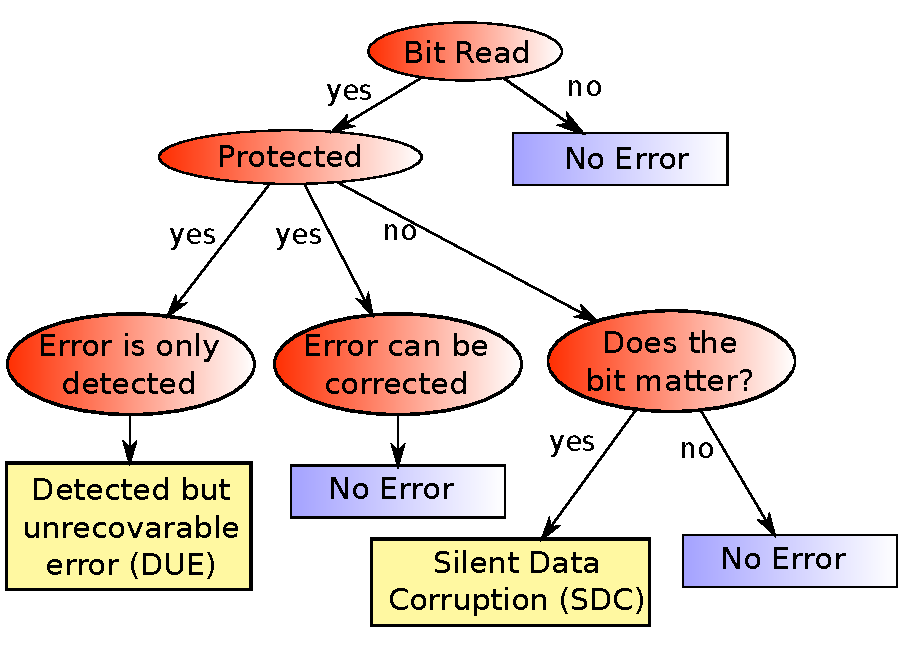
\includegraphics[width=3in]{sdc-due}
 \end{figure}
\end{center}

\begin{itemize}
 \item The error rate is a combination of SDC and DUE
\item SDC is potentially more harmful
\end{itemize}

\end{frame}

\begin{frame}[shrink=10]{Examples}
 \begin{example}{Example of SDC: }
  Bit flips in functional units that are not protected, e.g., ALU, decode logic, pipeline latches.
 \end{example}
 \begin{example}{Example of DUE: }
    Multiple SER  events in units that are protected like the register file or the caches.
 \end{example}

{\color{blue}{When is there no error?} } \\
\begin{columns}[t]
\pause
\begin{column}{0.6\textwidth}
Instructions that don't affect correctness
\begin{itemize}
 \item Dynamically dead instructions
 \item Wrong path instructions
  \item Performance instructions
  \item Prefetch instructions
  \item No ops
\end{itemize}
\end{column}
\pause
\begin{column}{0.4\textwidth}
Functional units that don't affect correctness
\begin{itemize}
 \item Branch predictor
  \item Performance counters
\end{itemize}
\end{column}

\end{columns}
\end{frame}

\begin{frame}[shrink=10]{AVF for Functional Units}
  \begin{itemize}
   \item {\color{blue} AVF} is typically calculated on a per functional unit basis
   \item It takes into cognizance the effect of redundant instructions, and characteristics of the functional unit.
      \begin{itemize}
       \item The AVF for the branch predictor is zero. 
      \item For the latches is about 50\%. 
	\item It varies widely from 10\% to 70\% for all other units.
      \end{itemize}
    \item How is AVF calculated?
      \begin{itemize}
	\item For units like the branch predictor, it can be calculated theoretically
	\item Otherwise, it is estimated with profiling runs for a set of benchmarks. 
	  \begin{itemize}
	    \item Inject a fault
	    \item Observe if the fault causes a failure in the program
	  \end{itemize}
      \end{itemize}
  \end{itemize}

\end{frame}

\begin{frame}[shrink=10]{Some More Definitions}
 \begin{definition}{ACE : }
  Architecturally Correct Execution. These are instructions that determine the program output. Their erroneous exeuction will
  lead to a failure.
 \end{definition}
\pause
\begin{definition}{Dynamically Dead Instruction : }
  These are instructions whose values don't propagate to the final output of the program. 
 \end{definition}

\pause
\begin{definition}{Ex-ACE instruction : }
  Let us consider an ACE instruction in the instruction queue. After it is issued, it is still in the queue till it gets
evicted by a newer instruction. After an ACE instruction leaves a functional unit, and is not required anymore by the unit, 
 it becomes an Ex-ACE instruction. 
\end{definition}

\end{frame}

\begin{frame}[shrink=10]{AVF for the Instruction Queue}
\begin{center}
\begin{figure}[h]
 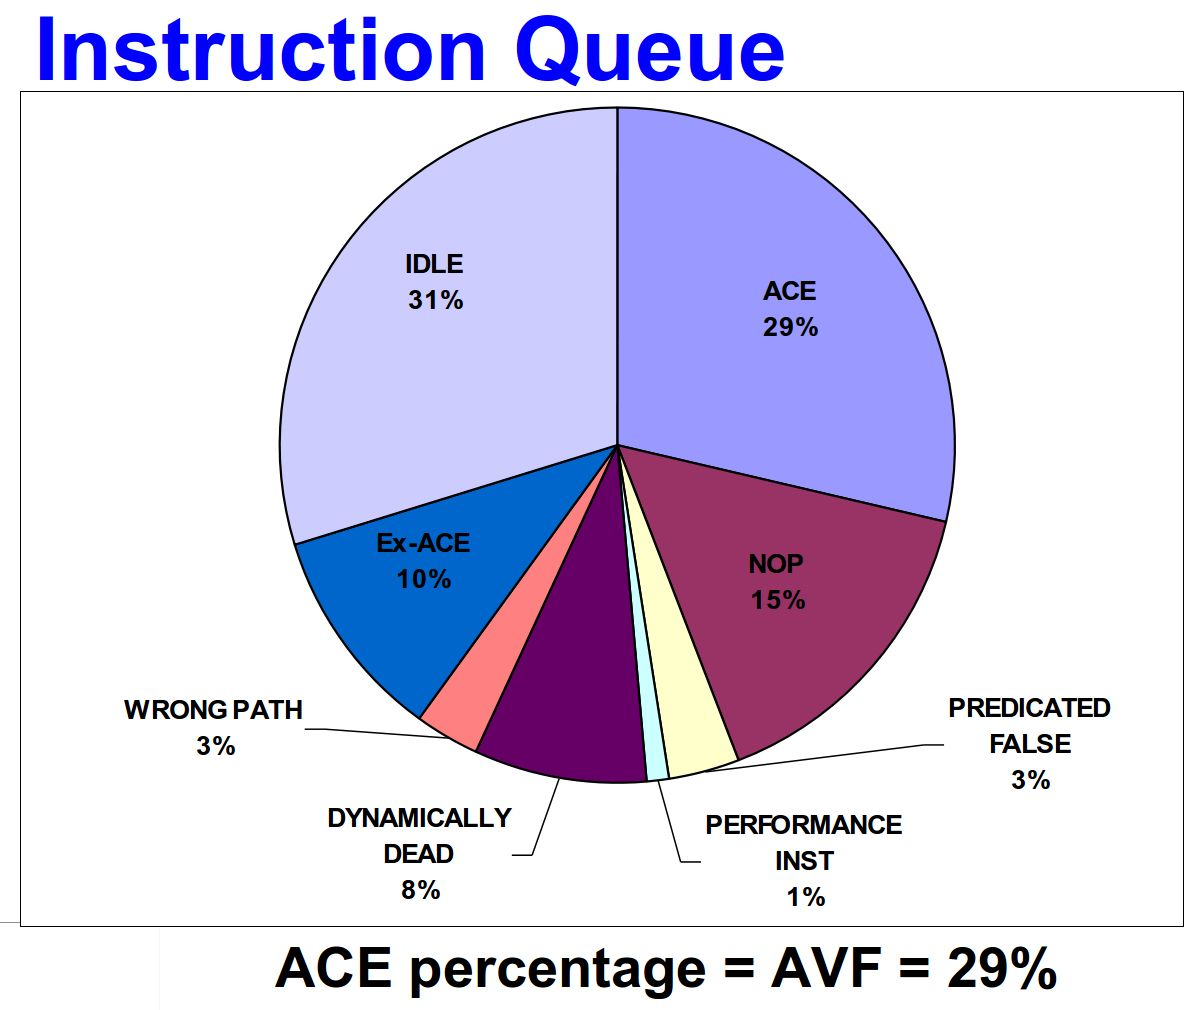
\includegraphics[width=3in]{inst_queue}
\caption{\footnotesize AVF for the instruction queue (courtesy Shubu Mukherjee Intel)}
\end{figure}
\end{center}
\end{frame}

% Bibliography
\bibliographystyle{plain}
\footnotesize
\begin{thebibliography}{10}
 \bibitem{shubu}
Shubhendu S. Mukherjee, 
Christopher T. Weaver, Joel S. Emer, Steven K. Reinhardt, Todd M. Austin: A Systematic 
Methodology to Compute the Architectural Vulnerability Factors for a High-Performance Microprocessor. MICRO 2003 \\
\url{http://portal.acm.org/citation.cfm?doid=956417.956570}

\bibitem{embedded}
Fan Wang, Agrawal, V.D. : Single Event Upset: An Embedded Tutorial, VLSI Design 2008 \\
\url{http://ieeexplore.ieee.org/xpls/abs_all.jsp?arnumber=4450538}

\end{thebibliography}

\end{document}